\documentclass[12pt,tikz]{standalone}

\usepackage{graphicx}
\usetikzlibrary{positioning}
\begin{document}
\fontsize{16}{20}\selectfont

\newcommand{\state}[2]{%
  $s = $ \texttt{#1}\\
  $p = $ \texttt{#2}
}

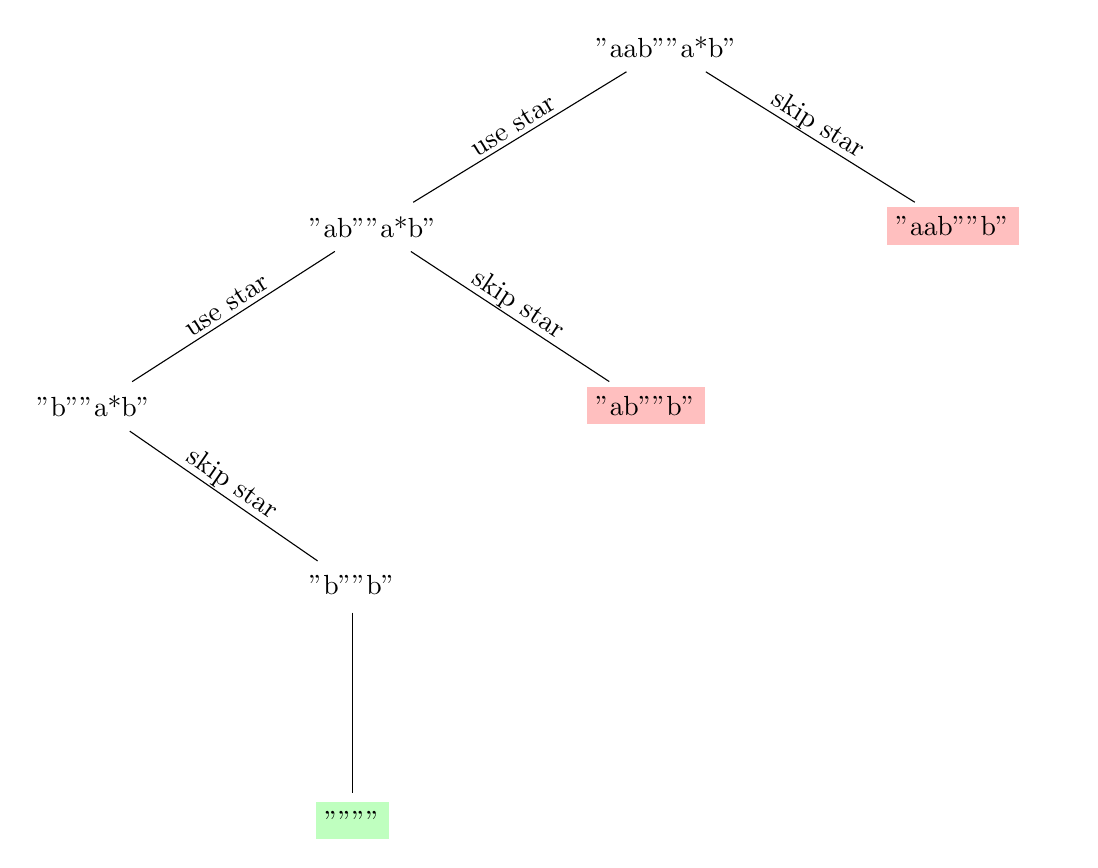
\begin{tikzpicture}[draw, black, shorten >=3pt, shorten <=3pt, node distance = 2.5cm]
  \node at (10, 0) (dummy) {};

  \node[align=center] (i0j0) at (5, 0) {\state{"aab"}{"a*b"}};

  \node[align=center, below left = of i0j0] (i1j0) {\state{"ab"}{"a*b"}};

  \draw (i0j0) to node[sloped, yshift=0.5em] (1) {use star} (i1j0);

  \node[fill=red!25, align=center, below right = of i0j0] (i0j2) {\state{"aab"}{"b"}};

  \draw (i0j0) to node[sloped, yshift=0.5em] (2) {skip star} (i0j2);

  \node[align=center, below left = of i1j0] (i2j0) {\state{"b"}{"a*b"}};

  \draw (i1j0) to node[sloped, yshift=0.5em] (3) {use star} (i2j0);

  \node[fill=red!25, align=center, below right = of i1j0] (i1j2) {\state{"ab"}{"b"}};

  \draw (i1j0) to node[sloped, yshift=0.5em] (4) {skip star} (i1j2);

  \node[align=center, below right = of i2j0] (i2j2) {\state{"b"}{"b"}};

  \draw (i2j0) to node[sloped, yshift=0.5em] (5) {skip star} (i2j2);

  \node[fill=green!25, align=center, below = of i2j2] (i3j3) {\state{""}{""}};

  \draw (i2j2) -- (i3j3);
\end{tikzpicture}

\end{document}
